\section{Covariance table generation}
\begin{frame}{Covariance table generation}
The covariance table $C$ is a data structure used to model the covariances in a grid. Each entry $C(hx,hy,hz)$ gives the covariance between points $p_1 = (x_1, y_1, z_1)$ and $p_2 = (x_2, y_2, z_2)$ apart $(hx, hy, hz)$, where $hx = x_2 - x_1$, $hy = y_2 - y_1$ and $hz = z_2 - z_1$.

There are two main ways to generate this table:
\begin{itemize}
	\item Implicit modeling: The data is used directly to generate the table. A smoothing strategy is needed to eliminate numeric artifacts and generate a positive-definite model\cite{cov.paper}.
    \item Explicit modeling: This is the traditional approach. An explicit model using admissible functions is used to fit a curve in an experimental variogram generated from data.
\end{itemize}
\end{frame}

\begin{frame}{The relationship between Covariance Table and Density Spectrum}
The density spectrum $s(\omega)$ is the Fourier Transform of the covariance table. As the covariance table is an even function, i. e., $C(h=(hx,hy,hz))=C(-h=(-hx,-hy,-hz))$, then the density spectrum is real and even.

$$
s(\omega)=\mathscr{F}\left[ C(h) \right]
$$
\end{frame}

\begin{frame}{The Bochner's Theorem}
An important result of the Theory of Fourier Transform is the Bochner's Theorem \cite{bochner1939additive}:

\begin{block}{}
A function $f(y)$ is positive-definite if it is the Fourier Transform of a real function $g(y) \geq 0$.
\end{block}
\end{frame}

\begin{frame}{Generating covariance tables using the Bochner's Theorem}
The Bochner's Theorem is an important tool to generate admissible covariance table from data, because the covariance table is a real function $C(h) \geq 0$.

Before generating the covariance table $C(h)$ is needed to build the experimental covariance table from data. This task can be done using the Marcotte approach \cite{fast.var.paper}, where Fast Fourier Transform (FFT) \cite{johnson2008implementing} is used to fast generation of experimental covariance table. Or the experimental covariance table can be generated using a geometric algorithm based on angular and bandwidth tolerances. 
\end{frame}


\begin{frame}{Generating covariance tables using the Bochner's Theorem}

\begin{itemize}
\item After generating the experimental covariance table $\tilde{C}(h)$, maybe some information is missing in some lags $h$ or there are many artifacts. In this case, it's needed to fill the missing data and remove the artifacts. An interpolation and smoothing algorithm is needed to adjust the experimental model $\tilde{C}(h)$ and generate an admissible covariance table $C(h)$. 

\item Yao \cite{cov.paper} presents an algorithm to execute the model interpolation and spectrum smoothing.
\end{itemize}

\end{frame}


\begin{frame}{The Yao's algorithm}

\begin{enumerate}
\item Let $\tilde{C}(h)$ an interpolated experimental covariance model generated using the data. The used interpolation can be a radial inverse distance interpolation or other type of interpolation based on distance. The interpolation is the first step to smooth the covariance model and remove artifacts. But, this interpolation doesn't assure a smooth positive definite model.
\item $\tilde{C}(h)$ is even and real. Then the Bochner's Theorem can be used.
\item Let $\tilde{s}(\omega)$ the density spectrum of $\tilde{C}(h)$. To generate a positive-definite function $C(h)$ is enough to smooth $\tilde{s}(\omega)$ using a moving average in each point of the density spectrum $\tilde{s}(\omega)$. 
\item Let $s(\omega)$ the smoothed density spectrum generated in the previous step. Applying the Inverse Fourier Transform $\mathscr{F}^{-1}$ in $s$, an admissible covariance table $C(h) = \mathscr{F}^{-1}[s(\omega)]$ is generated.
\end{enumerate}

\end{frame}

\begin{frame}{A covariance table figure}

\begin{figure}[!ht]
  \caption{A smoothed covariance table generated using the Walker Lake data-set and the Yao's algorithm.}
  \centering
    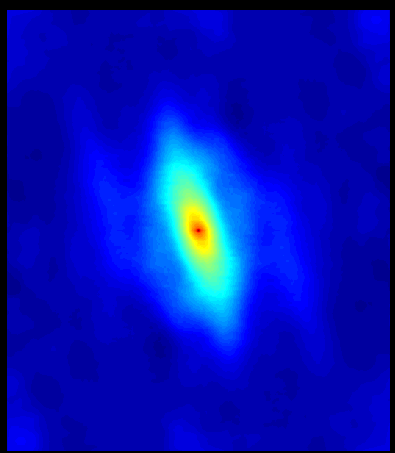
\includegraphics[height=0.4\textheight, width=0.6\textwidth]{figs/cov_table_fig.png}
    \label{cov_table_ex.fig}
\end{figure}

\end{frame}

\begin{frame}{A density spectrum figure}
\begin{figure}[!ht]
  \caption{A smoothed density spectrum generated using the Walker Lake data-set and the Yao's algorithm.}
  \centering
    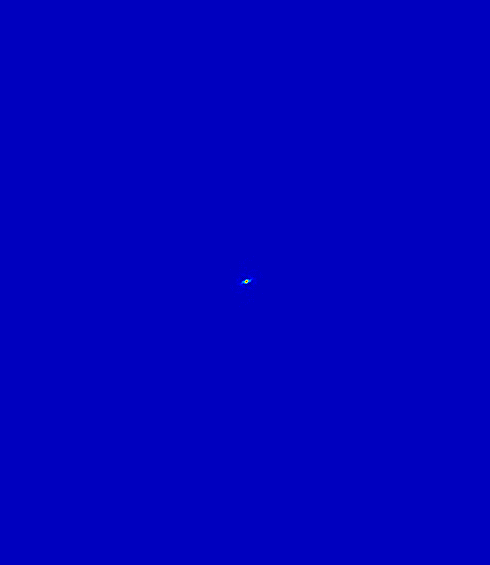
\includegraphics[height=0.5\textheight]{figs/dens_spec.png}
    \label{dens_spec.fig}
\end{figure}
\end{frame}


\begin{frame}{Why covariance tables are useful?}
\begin{itemize}
\item The covariance table $C(h)$ can be used in traditional simulation/estimation algorithms like Sequential Gaussian Simulation, Kriging and so on.
\item It can be used in the post-conditioning step of spectral simulations like Turning Bands and Fourier Integral Method.
\item The covariance modeling is the most human-time expense stage of the geostatistical modeling. A semi-automatic covariance table modeling tool could save this time. Mainly, when a multi-variate model is being built \cite{cov.paper}.
\end{itemize}
\end{frame}

\begin{frame}{The covariance table modeling challenges}

\begin{itemize}
\item The Yao's algorithm is a powerful technique. But, it's highly dependent of the quality of input data. It demands a good sampling of simulation/estimation domain.

\item To lead with this limitation an explicit model is needed or an auxiliary  model containing the expected covariance is needed.

\item How to generate this auxiliary model? Using Radial Base Functions? Using some machine learning estimation technique?

\item This is an open question to be answered.
\end{itemize}

\end{frame}


